\documentclass[slovene,11pt,a4paper]{article}
\usepackage[margin=2cm,bottom=2cm,foot=1.5cm]{geometry}
% \documentclass[slovene,11pt,a4paper]{article}
% \usepackage[margin=1.7cm,bottom=3cm,foot=1.5cm]{geometry}
\setlength{\parindent}{0pt}
\setlength{\parskip}{0.5ex}

\usepackage[pdftex]{graphicx}
\usepackage{pgffor}
\usepackage{subcaption}
% \usepackage{a4wide} %najaci package
\usepackage[utf8]{inputenc}
\usepackage[slovene]{babel}
\usepackage{color}
\usepackage{graphicx}
% \usepackage{subfigure}
\usepackage{imakeidx}
\usepackage{adjustbox}
\usepackage{float}
\usepackage{amsmath}
\usepackage{mathtools}
\usepackage{tikz}
\usepackage{amssymb}
\usepackage{listings}
\usepackage{siunitx}
\usepackage{hyperref}
\usepackage{amsfonts}
\usepackage{mathrsfs}


%\def\phi{\phi}
\def\eps{\varepsilon}
\def\theta{\vartheta}

\newcommand{\thisyear}{2024/25}

\renewcommand{\Re}{\mathop{\rm Re}\nolimits}
\renewcommand{\Im}{\mathop{\rm Im}\nolimits}
\newcommand{\Tr}{\mathop{\rm Tr}\nolimits}
\newcommand{\diag}{\mathop{\rm diag}\nolimits}
\newcommand{\dd}{\,\mathrm{d}}
\newcommand{\ddd}{\mathrm{d}}
\newcommand{\ii}{\mathrm{i}}
\newcommand{\lag}{\mathcal{L}\!}
\newcommand{\ham}{\mathcal{H}\!}
\newcommand{\four}[1]{\mathcal{F}\!\left(#1\right)}
\newcommand{\bigO}[1]{\mathcal{O}\!\left(#1\right)}
\newcommand{\sh}{\mathop{\rm sinh}\nolimits}
\newcommand{\ch}{\mathop{\rm cosh}\nolimits}
\renewcommand{\th}{\mathop{\rm tanh}\nolimits}
\newcommand{\erf}{\mathop{\rm erf}\nolimits}
\newcommand{\erfc}{\mathop{\rm erfc}\nolimits}
\newcommand{\sinc}{\mathop{\rm sinc}\nolimits}
\newcommand{\rect}{\mathop{\rm rect}\nolimits}
\newcommand{\ee}[1]{\cdot 10^{#1}}
\newcommand{\inv}[1]{\left(#1\right)^{-1}}
\newcommand{\invf}[1]{\frac{1}{#1}}
\newcommand{\sqr}[1]{\left(#1\right)^2}
\newcommand{\half}{\frac{1}{2}}
\newcommand{\thalf}{\tfrac{1}{2}}
\newcommand{\pd}{\partial}
\newcommand{\Dd}[3][{}]{\frac{\ddd^{#1} #2}{\ddd #3^{#1}}}
\newcommand{\Pd}[3][{}]{\frac{\pd^{#1} #2}{\pd #3^{#1}}}
\newcommand{\avg}[1]{\left\langle#1\right\rangle}
\newcommand{\norm}[1]{\left\Vert #1 \right\Vert}
\newcommand{\braket}[2]{\left\langle #1 \vert#2 \right\rangle}
\newcommand{\obraket}[3]{\left\langle #1 \vert #2 \vert #3 \right \rangle}
\newcommand{\hex}[1]{\texttt{0x#1}}

\renewcommand{\iint}{\mathop{\int\mkern-13mu\int}}
\renewcommand{\iiint}{\mathop{\int\mkern-13mu\int\mkern-13mu\int}}
\newcommand{\oiint}{\mathop{{\int\mkern-15mu\int}\mkern-21mu\raisebox{0.3ex}{$\bigcirc$}}}

\newcommand{\wunderbrace}[2]{\vphantom{#1}\smash{\underbrace{#1}_{#2}}}

\newcommand{\bec}[1]{\mathbf{#1}}


\title{
\sc\large Matematično-fizikalni praktikum \thisyear\\
\bigskip
\bf\Large 11.~naloga: Reševanje PDE z metodo Galerkina
}
\author{Tadej Tomažič}
\date{}

\makeindex[columns=3, title=Alphabetical Index, intoc]

\begin{document}


\pagenumbering{gobble} 
\author{Tadej Tomažič}
\date{\today}

\maketitle

\newpage
\pagenumbering{arabic}
\tableofcontents
\listoffigures
\newpage
\vspace{-1cm}
\section{Navodilo}



Pri opisu enakomernega laminarnega toka viskozne in nestisljive
tekočine po dolgi ravni cevi pod vplivom stalnega tlačnega
gradienta $p^{\prime}$ se Navier-Stokesova enačba poenostavi
v Poissonovo enačbo
\begin{equation*}
  \nabla^2 v = \Delta v = - \frac{p^\prime}{\eta}\>,
\end{equation*}
kjer je $v$ vzdolžna komponenta hitrosti, odvisna samo  od
koordinat preseka cevi, $\eta$ pa je viskoznost tekočine.
Enačbo rešujemo v notranjosti preseka cevi, medtem ko
je ob stenah hitrost tekočina enaka nič.  Za pretok velja
Poiseuillov zakon
\begin{equation*}
  \Phi = \int_S v\dd S = C\,\frac{p' S^2}{ 8\pi\eta} \>,
\end{equation*}
kjer je koeficient $C$ odvisen samo od oblike preseka cevi
($C=1$ za okroglo cev).  Določili bomo koeficient za
polkrožno cev z radijem $R$. V novih spremenljivkah $\xi=r/R$
in $u=v \eta/(p^\prime R^2)$ se problem glasi
\begin{equation*}
\Delta u(\xi,\phi) = -1 \>,\qquad
u(\xi=1,\phi)=u(\xi,0)=u(\xi,\phi=\pi)=0 \>,
\end{equation*}
\begin{equation*}
  C = 8\pi \iint \frac{u(\xi,\phi)\,\xi\dd \xi \dd\phi}{ (\pi/2)^2} \>.
\end{equation*}

Če poznamo lastne funkcije diferencialnega operatorja za določeno
geometrijo\footnote{Spomni se na primer na vodikov atom v sferični geometriji,
kjer smo imeli $\widehat{L}^2 Y_{lm}(\theta,\phi) = \hbar^2 l(l+1)
Y_{lm}(\theta,\phi)$ in $\widehat{L}_z Y_{lm}(\theta,\phi) = m \hbar
Y_{lm}(\theta,\phi)$.} se reševanje parcialnih diferencialnih enačb
včasih lahko prevede na razvoj po lastnih funkcijah. Da bi se izognili
računanju lastnih (za ta primer Besselovih) funkcij in njihovih ničel,
ki jih potrebujemo v razvoju, lahko zapišemo aproksimativno
rešitev kot linearno kombinacijo nekih poskusnih ({\sl trial\/})
funkcij
\begin{equation}
\tilde{u}(\xi,\phi) = \sum\limits_{i=1}^N  a_i \Psi_i(\xi,\phi),
\label{eq:trials}
\end{equation}
za katere ni nujno, da so ortogonalne, pač pa naj zadoščajo
robnim pogojem, tako da jim bo avtomatično zadoščala tudi
vsota (\ref{eq:trials}). Ta pristop nam pride prav v kompleksnejših geometrijah,
ko je uporabnost lastnih funkcij izključena in potrebujemo robustnejši pristop.
Približna funkcija $\tilde{u}$ seveda ne zadosti Poissonovi enačbi: preostane majhna napaka $\varepsilon$
\begin{equation*}
  \Delta \tilde{u}(\xi,\phi) + 1 = \varepsilon(\xi,\phi) \>.
\end{equation*}
Pri metodi Galerkina zahtevamo, da je napaka ortogonalna
na vse poskusne funkcije $\Psi_i$,
\begin{equation*}
  (\varepsilon,\Psi_i) = 0 \>, \qquad  i = 1,2,\dots, N \>.
\end{equation*}
V splošnem bi lahko zahtevali tudi ortogonalnost $\varepsilon$
na nek drug sistem utežnih ({\sl weight\/}) oziroma testnih
({\sl test\/}) funkcij $\Psi_i$.  Metoda Galerkina je poseben
primer takih metod ({\sl Methods of Weighted Residuals\/})
z izbiro $\Psi_i = \Psi_i$.  Omenjena izbira vodi do sistema
enačb za koeficiente $a_i$
\begin{equation}
  \sum_{j=1}^N A_{ij} a_j = b_i\>, \qquad  i = 1,2,\dots, N \>,
  \label{eq:sistem}
\end{equation}
\[
A_{ij} = (\Delta \Psi_j,\Psi_i) \>, \qquad b_i = (-1,\Psi_i) \>,
\]
tako da je koeficient za pretok enak
\begin{equation*}
C =-\frac{32}{ \pi} \sum_{ij}  b_i A_{ij}^{-1} b_j \>.
\end{equation*}
Za kotni del poskusne funkcije obdržimo eksaktne funkcije
$\sin((2m+1)\phi)$, Besselove funkcije za radialni del
pa nadomestimo s preprostejšimi funkcijami $\xi^{2m+1}(1-\xi)^n$.
Pozor: indeks $i$ pomeni seveda dvojni indeks (šteje obenem
$m$ in $n$)\footnote{Glej tudi prilogo na spletni učilnici.}.  Zaradi ortogonalnosti po $m$ razpade matrika $A$ v bloke,
obrneš pa jo lahko s kako pripravljeno rutino, npr. s spodnjim
in zgornjim trikotnim razcepom {\tt ludcmp} in {\tt lubksb} iz NRC.

\bigskip

{\sl Naloga:} 
Izračunaj koeficient $C$.  V ta namen moraš dobiti matriko $A$
in vektor $b$; preuči, kako je natančnost rezultata
(vsote za koeficient $C$) odvisna od števila členov
v indeksih $m$ in $n$. Zaradi ortogonalnosti
po $m$ lahko oba učinka preučuješ neodvisno.

\bigskip

{\sl Dodatna naloga:}  V praksi je metoda Galerkina primerna
v zapletenih geometrijah, ko grobe ocene dobimo že z eno samo
(ali le nekaj) dobro izbranimi poskusnimi funkcijami,
in ko še ni pretežko obrniti sistema~(\ref{eq:sistem}).
če pa želimo uporabiti metodo izčrpneje,
za večjo natančnost, si težko izmislimo dovolj
bogat izbor funkcij $\Psi$.

Da ima metoda Galerkina določene prednosti celo pred preprostimi
diferenčnimi metodami, opazujmo še na primeru linearne hiperbolične
valovne enačbe v eni dimenziji
\begin{equation*}
  \frac{\partial u}{\partial t} - \frac{\partial u}{\partial \xi} = 0
\end{equation*}
za $\xi \in[0,2\pi]$ s periodičnimi robnimi pogoji.
Začetni pogoj naj bo $u(\xi,0)=\sin(\pi\cos \xi)$;
analitična rešitev enačbe je $u(\xi,t)=\sin(\pi\cos(\xi+t))$.
Približno rešitev formalno razvijemo po poskusnih funkcijah
\begin{equation}
  \widetilde{u}(\xi,t) = \sum_{j=-N/2}^{N/2} a_j(t) \Psi_j(\xi)
  \label{eq:razvoj}
\end{equation}
in po Galerkinu zahtevamo
\begin{equation}
\int_0^{2\pi} \left[ \Pd{\widetilde{u}}{t} -
  \Pd{\widetilde{u}}{\xi} \right] \Psi^*_k(\xi) \dd \xi = 0 \>.
\label{eq:zahteva}
\end{equation}
Najočitnejša izbira je ravni val po kraju $\Psi_j(\xi) = \frac{1}{\sqrt{2\pi}} \mathrm{e}^{\mathrm{i}j\xi}$ in 
skalarni produkt v kompleksnem 
\begin{equation}
 \left( \Psi_k, \Psi_j \right) = \int_{0}^{2\pi} \Psi^*_k(\xi) \Psi_j(\xi) \, \mathrm{d}\xi =  \frac{1}{2\pi} \int_{0}^{2\pi} e^{-i k \xi} e^{i j \xi} \, \mathrm{d}\xi = \delta_{jk},
\label{eq:skalarni}
\end{equation}
 tako da imamo
obenem tudi ortonormalnost.  Funkcijo $u(\xi,t)$ seveda še iščemo:
določi jo ravno Galerkinova zahteva~(\ref{eq:zahteva}), iz katere sledi
sistem sklopljenih enačb za koeficiente $a_k(t)$
\begin{equation}
\Dd{a_k}{t} - \mathrm{i}ka_k = 0 \>, \qquad
k = -N/2, \dots, N/2 \>.
\label{eq:koeficienti}
\end{equation}
Začetni pogoj za ta sistem so vrednosti
\begin{equation*}
  a_k(0) = \int_0^{2\pi} u(\xi,0) \Psi^*_k(\xi) \dd \xi \>.
\end{equation*}
Za izračun $a_k(0)$ in časovni razvoj sistema enačb~(\ref{eq:koeficienti})
uporabi kak preverjeni integrator, na primer RK4, in ob
izbranih časih poišči rešitev~(\ref{eq:razvoj}).  Za kontrolo imaš
lahko koeficiente razvoja analitične rešitve, ki so
\begin{equation*}
  a_k(t)=\sin\left(\frac{k\pi}{ 2}\right)\,J_k(\pi)\,\mathrm{e}^{\mathrm{i}kt} \>.
\end{equation*}
Za negativne indekse Besselovih funkcij uporabi zvezo
$J_{-\nu} = \cos(\nu\pi) J_\nu - \sin(\nu\pi) Y_\nu$.
Primerjaj dobljeni rezultat s tistim, ki ga dobiš,
če prvotno parcialno diferencialno enačbo diskretiziraš
v prvem redu
\begin{equation*}
\frac{u_{i+1,j} - u_{i,j}}{ k} = \frac{u_{i,j+1} - u_{i,j}}{ h}
\end{equation*}
in to rešuješ v času naprej eksplicitno kot
$u_{i+1,j} = u_{i,j} + (k/h)(u_{i,j+1} - u_{i,j})$.
\section{Rešitev}

Najprej si poglejmo avtokorelacijo za obe sovi.
\begin{figure}[h]
    \centering
    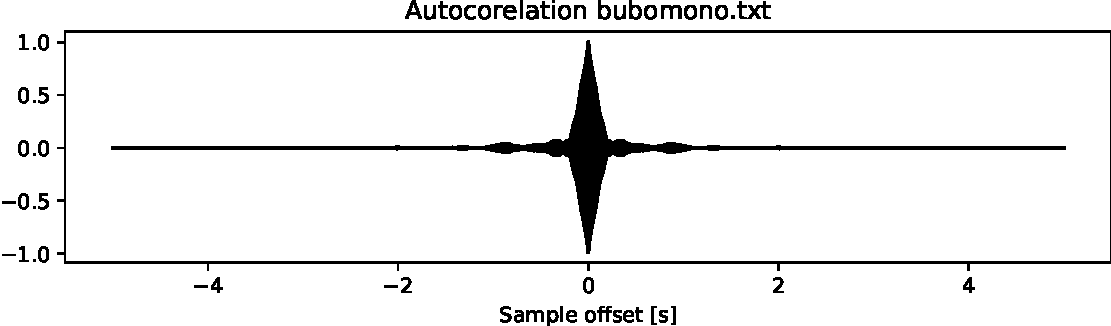
\includegraphics[width=12cm]{pdfs/bubomono.txt_acor.pdf}
    \vspace{10pt}
    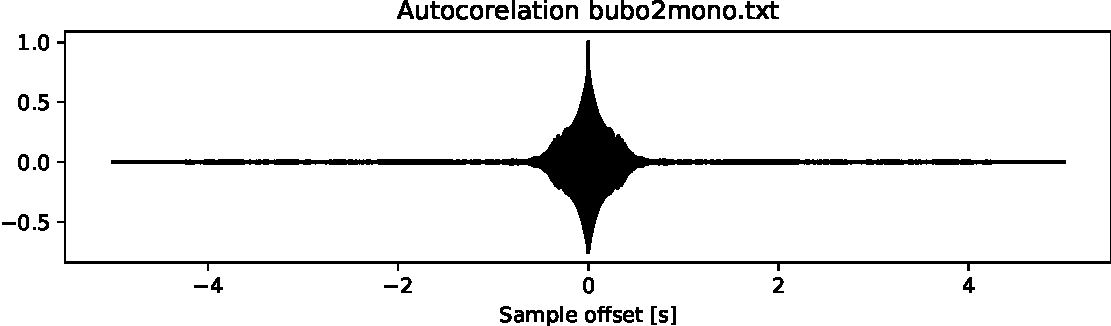
\includegraphics[width=12cm]{pdfs/bubo2mono.txt_acor.pdf}
    \caption{Avtokorelacija signala sov}
\end{figure}

Preden sem koreliral signal sem vektorja samplov normiral, tako da je
"najmočnejši" signal 1. To pomeni \[\|x\|_\infty = \max_i |x_i|\]

Poglejmo si še korelacije med sovami in posnetki:
\newpage
\begin{figure}[h]
    \centering
    \foreach \mix in {mix, mix1, mix2, mix22} {
        \foreach \sova in {bubomono, bubo2mono}{
            \includegraphics[width=8cm]{pdfs/cor_\mix.txt_\sova.txt.pdf}
        }
    }
    \caption{Korelacija sov in posnetkov iz narave}
\end{figure}
Tukaj je bila normalizacija drugače izbrana. Tukaj je bila narejena normalizacija korelacije. Če je varianca signala a $\sigma_a$,
potem je $ \mathbf{x} = \mathbf{x} / \left(\sigma_a \sigma_b |\mathbf{b}|\right)$. Sigma je izračunana z \verb|numpy.std()|.


Hitrosti so precej dolgčasno pričakovane ampak vseeno.
\begin{figure}[h]
    \centering
    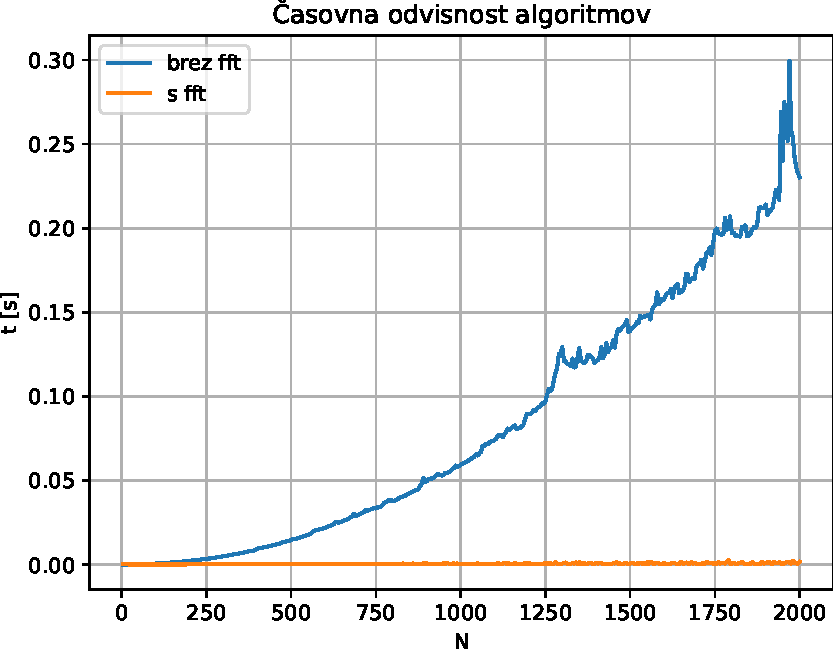
\includegraphics[width=8cm]{pdfs/cas-lin.pdf}
    \vspace{10pt}
    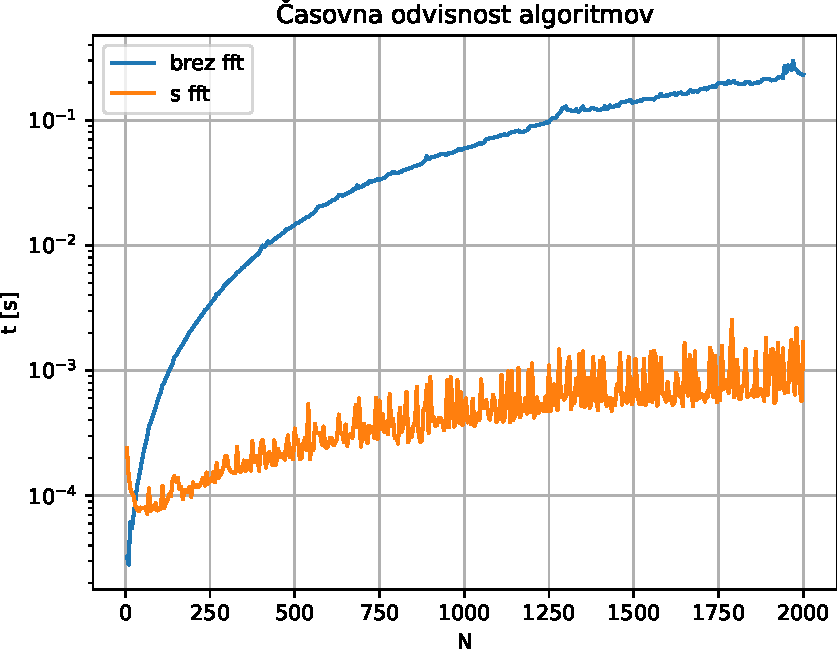
\includegraphics[width=8cm]{pdfs/cas-log.pdf}
    \caption{Hitrost algoritmov}
\end{figure}
\newpage
\section{Dodatna naloga}
Posnel sem dva človeka m in ž ko izgovarjata aaaaaaaaaaaa. Posnel sem jih tudi
ko bereta slovar. Gledal sem ali lahko spet zaznam ali gre za ž glas ali m glas.
Poglejmo si spektra njunega glasu.
\begin{figure}[h]
    \begin{center}
        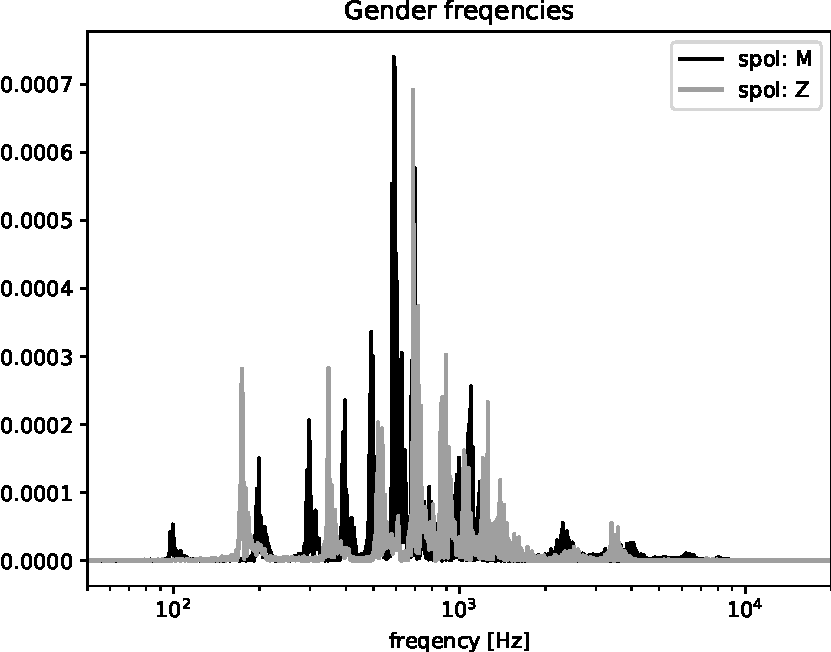
\includegraphics[width=12cm]{pdfs/fft_spol.pdf}
    \end{center}
    \caption{Barva glasu moškega in ženske}
\end{figure}

% Glasova sta bila prej normirana, saj je bil moški glas posnet bližje mikrofona.
% Poglejmo si zopet korelacijo med posnetki:
% \foreach \gender in {Z, M} {
%     \foreach \mix in {Glas\ 001, Glas\ 002}{
%         pdfs/cor_\gender_\mix.pdf 
%     }
% }
\begin{figure}[h]
    \begin{center}
        
    \foreach \gender in {Z, M} {%
        \foreach \mix in {001, 002} {%
            \includegraphics[width=8cm]{pdfs/cor_\gender_Glas\space\mix.pdf}%    
        }%
        \par
}%
    \end{center}
    
    \caption{Korelacija glasa človeka in posnetkov iz branja slovarja}
\end{figure}

\end{document}
